\documentclass[8pt]{beamer}

% Beamer style
%\usetheme[secheader]{Madrid}
% \usetheme{CambridgeUS}
\useoutertheme{infolines}
\usecolortheme[rgb={0.65,0.15,0.25}]{structure}
% \usefonttheme[onlymath]{serif}
\beamertemplatenavigationsymbolsempty
%\AtBeginSubsection

% Packages
%\usepackage[french]{babel}
\usepackage[latin1]{inputenc}
\usepackage{color}
% \usepackage[dvipsnames]{xcolor}
\usepackage{xspace}
\usepackage{dsfont, stmaryrd}
\usepackage{amsmath, amsfonts, amssymb, stmaryrd, mathabx}
\usepackage{epsfig}
\usepackage{tikz}
\usepackage{url}
% \usepackage{ulem}
\usepackage{/home/robin/LATEX/Biblio/astats}
%\usepackage[all]{xy}
\usepackage{graphicx}

% Maths
% \newtheorem{theorem}{Theorem}
% \newtheorem{definition}{Definition}
\newtheorem{proposition}{Proposition}
% \newtheorem{assumption}{Assumption}
% \newtheorem{algorithm}{Algorithm}
% \newtheorem{lemma}{Lemma}
% \newtheorem{remark}{Remark}
% \newtheorem{exercise}{Exercise}
% \newcommand{\propname}{Prop.}
% \newcommand{\proof}{\noindent{\sl Proof:}\quad}
% \newcommand{\eproof}{$\blacksquare$}

% \setcounter{secnumdepth}{3}
% \setcounter{tocdepth}{3}
\newcommand{\pref}[1]{\ref{#1} p.\pageref{#1}}
\newcommand{\qref}[1]{\eqref{#1} p.\pageref{#1}}

% Colors : http://latexcolor.com/
\definecolor{darkred}{rgb}{0.65,0.15,0.25}
\definecolor{darkgreen}{rgb}{0,0.4,0}
\definecolor{darkred}{rgb}{0.65,0.15,0.25}
\definecolor{amethyst}{rgb}{0.6, 0.4, 0.8}
\definecolor{asparagus}{rgb}{0.53, 0.66, 0.42}
\definecolor{applegreen}{rgb}{0.55, 0.71, 0.0}
\definecolor{awesome}{rgb}{1.0, 0.13, 0.32}
\definecolor{blue-green}{rgb}{0.0, 0.87, 0.87}
\definecolor{red-ggplot}{rgb}{0.52, 0.25, 0.23}
\definecolor{green-ggplot}{rgb}{0.42, 0.58, 0.00}
\definecolor{purple-ggplot}{rgb}{0.34, 0.21, 0.44}
\definecolor{blue-ggplot}{rgb}{0.00, 0.49, 0.51}

% Commands
\newcommand{\backupbegin}{
   \newcounter{finalframe}
   \setcounter{finalframe}{\value{framenumber}}
}
\newcommand{\backupend}{
   \setcounter{framenumber}{\value{finalframe}}
}
\newcommand{\emphase}[1]{\textcolor{darkred}{#1}}
\newcommand{\comment}[1]{\textcolor{gray}{#1}}
\newcommand{\paragraph}[1]{\textcolor{darkred}{#1}}
\newcommand{\refer}[1]{{\small{\textcolor{gray}{{\cite{#1}}}}}}
\newcommand{\Refer}[1]{{\small{\textcolor{gray}{{[#1]}}}}}
\newcommand{\goto}[1]{{\small{\textcolor{blue}{[\#\ref{#1}]}}}}
\renewcommand{\newblock}{}

\newcommand{\tabequation}[1]{{\medskip \centerline{#1} \medskip}}
% \renewcommand{\binom}[2]{{\left(\begin{array}{c} #1 \\ #2 \end{array}\right)}}

% Variables 
\newcommand{\Abf}{{\bf A}}
\newcommand{\Beta}{\text{B}}
\newcommand{\Bcal}{\mathcal{B}}
\newcommand{\Bias}{\xspace\mathbb B}
\newcommand{\Cor}{{\mathbb C}\text{or}}
\newcommand{\Cov}{{\mathbb C}\text{ov}}
\newcommand{\cl}{\text{\it c}\ell}
\newcommand{\Ccal}{\mathcal{C}}
\newcommand{\cst}{\text{cst}}
\newcommand{\Dcal}{\mathcal{D}}
\newcommand{\Ecal}{\mathcal{E}}
\newcommand{\Esp}{\xspace\mathbb E}
\newcommand{\Espt}{\widetilde{\Esp}}
\newcommand{\Covt}{\widetilde{\Cov}}
\newcommand{\Ibb}{\mathbb I}
\newcommand{\Fcal}{\mathcal{F}}
\newcommand{\Gcal}{\mathcal{G}}
\newcommand{\Gam}{\mathcal{G}\text{am}}
\newcommand{\Hcal}{\mathcal{H}}
\newcommand{\Jcal}{\mathcal{J}}
\newcommand{\Lcal}{\mathcal{L}}
\newcommand{\Mt}{\widetilde{M}}
\newcommand{\mt}{\widetilde{m}}
\newcommand{\Nbb}{\mathbb{N}}
\newcommand{\Mcal}{\mathcal{M}}
\newcommand{\Ncal}{\mathcal{N}}
\newcommand{\Ocal}{\mathcal{O}}
\newcommand{\pt}{\widetilde{p}}
\newcommand{\Pt}{\widetilde{P}}
\newcommand{\Pbb}{\mathbb{P}}
\newcommand{\Pcal}{\mathcal{P}}
\newcommand{\Qcal}{\mathcal{Q}}
\newcommand{\qt}{\widetilde{q}}
\newcommand{\Rbb}{\mathbb{R}}
\newcommand{\Sbb}{\mathbb{S}}
\newcommand{\Scal}{\mathcal{S}}
\newcommand{\st}{\widetilde{s}}
\newcommand{\St}{\widetilde{S}}
\newcommand{\Tcal}{\mathcal{T}}
\newcommand{\todo}{\textcolor{red}{TO DO}}
\newcommand{\Ucal}{\mathcal{U}}
\newcommand{\Un}{\math{1}}
\newcommand{\Vcal}{\mathcal{V}}
\newcommand{\Var}{\mathbb V}
\newcommand{\Vart}{\widetilde{\Var}}
\newcommand{\Zcal}{\mathcal{Z}}

% Symboles & notations
\newcommand\independent{\protect\mathpalette{\protect\independenT}{\perp}}\def\independenT#1#2{\mathrel{\rlap{$#1#2$}\mkern2mu{#1#2}}} 
\renewcommand{\d}{\text{\xspace d}}
\newcommand{\gv}{\mid}
\newcommand{\ggv}{\, \| \, }
% \newcommand{\diag}{\text{diag}}
\newcommand{\card}[1]{\text{card}\left(#1\right)}
\newcommand{\trace}[1]{\text{tr}\left(#1\right)}
\newcommand{\matr}[1]{\boldsymbol{#1}}
\newcommand{\matrbf}[1]{\mathbf{#1}}
\newcommand{\vect}[1]{\matr{#1}} %% un peu inutile
\newcommand{\vectbf}[1]{\matrbf{#1}} %% un peu inutile
\newcommand{\trans}{\intercal}
\newcommand{\transpose}[1]{\matr{#1}^\trans}
\newcommand{\crossprod}[2]{\transpose{#1} \matr{#2}}
\newcommand{\tcrossprod}[2]{\matr{#1} \transpose{#2}}
\newcommand{\matprod}[2]{\matr{#1} \matr{#2}}
\DeclareMathOperator*{\argmin}{arg\,min}
\DeclareMathOperator*{\argmax}{arg\,max}
\DeclareMathOperator{\sign}{sign}
\DeclareMathOperator{\tr}{tr}
\newcommand{\ra}{\emphase{$\rightarrow$} \xspace}

% Hadamard, Kronecker and vec operators
\DeclareMathOperator{\Diag}{Diag} % matrix diagonal
\DeclareMathOperator{\diag}{diag} % vector diagonal
\DeclareMathOperator{\mtov}{vec} % matrix to vector
\newcommand{\kro}{\otimes} % Kronecker product
\newcommand{\had}{\odot}   % Hadamard product

% TikZ
\newcommand{\nodesize}{2em}
\newcommand{\edgeunit}{2.5*\nodesize}
\newcommand{\edgewidth}{1pt}
\tikzstyle{node}=[draw, circle, fill=black, minimum width=.75\nodesize, inner sep=0]
\tikzstyle{square}=[rectangle, draw]
\tikzstyle{param}=[draw, rectangle, fill=gray!50, minimum width=\nodesize, minimum height=\nodesize, inner sep=0]
\tikzstyle{hidden}=[draw, circle, fill=gray!50, minimum width=\nodesize, inner sep=0]
\tikzstyle{hiddenred}=[draw, circle, color=red, fill=gray!50, minimum width=\nodesize, inner sep=0]
\tikzstyle{observed}=[draw, circle, minimum width=\nodesize, inner sep=0]
\tikzstyle{observedred}=[draw, circle, minimum width=\nodesize, color=red, inner sep=0]
\tikzstyle{eliminated}=[draw, circle, minimum width=\nodesize, color=gray!50, inner sep=0]
\tikzstyle{empty}=[draw, circle, minimum width=\nodesize, color=white, inner sep=0]
\tikzstyle{blank}=[color=white]
\tikzstyle{nocircle}=[minimum width=\nodesize, inner sep=0]

\tikzstyle{edge}=[-, line width=\edgewidth]
\tikzstyle{edgebendleft}=[-, >=latex, line width=\edgewidth, bend left]
\tikzstyle{edgebendright}=[-, >=latex, line width=\edgewidth, bend right]
\tikzstyle{lightedge}=[-, line width=\edgewidth, color=gray!50]
\tikzstyle{lightedgebendleft}=[-, >=latex, line width=\edgewidth, bend left, color=gray!50]
\tikzstyle{lightedgebendright}=[-, >=latex, line width=\edgewidth, bend right, color=gray!50]
\tikzstyle{edgered}=[-, line width=\edgewidth, color=red]
\tikzstyle{edgebendleftred}=[-, >=latex, line width=\edgewidth, bend left, color=red]
\tikzstyle{edgebendrightred}=[-, >=latex, line width=\edgewidth, bend right, color=red]

\tikzstyle{arrow}=[->, >=latex, line width=\edgewidth]
\tikzstyle{arrowbendleft}=[->, >=latex, line width=\edgewidth, bend left]
\tikzstyle{arrowbendright}=[->, >=latex, line width=\edgewidth, bend right]
\tikzstyle{arrowred}=[->, >=latex, line width=\edgewidth, color=red]
\tikzstyle{arrowbendleftred}=[->, >=latex, line width=\edgewidth, bend left, color=red]
\tikzstyle{arrowbendrightred}=[->, >=latex, line width=\edgewidth, bend right, color=red]
\tikzstyle{arrowblue}=[->, >=latex, line width=\edgewidth, color=blue]
\tikzstyle{dashedarrow}=[->, >=latex, dashed, line width=\edgewidth]
\tikzstyle{dashededge}=[-, >=latex, dashed, line width=\edgewidth]
\tikzstyle{dashededgebendleft}=[-, >=latex, dashed, line width=\edgewidth, bend left]
\tikzstyle{lightarrow}=[->, >=latex, line width=\edgewidth, color=gray!50]

\newcommand{\dN}{\Delta N}
\newcommand{\dtau}{\Delta \tau}

% Directory
\newcommand{\fig}{/home/robin/RECHERCHE/ECOLOGIE/EXPOSES/FIGURES}
\newcommand{\figeco}{\fig}
\newcommand{\fignet}{/home/robin/RECHERCHE/RESEAUX/EXPOSES/FIGURES}
\newcommand{\figbayes}{/home/robin/RECHERCHE/BAYES/EXPOSES/FIGURES}
% \newcommand{\figDoR}{/home/robin/RECHERCHE/BAYES/VBEM-IS/VBEM-IS.git/Paper/JRSSC-V3/Figs}

%====================================================================
%====================================================================

%====================================================================
%====================================================================
\begin{document}
%====================================================================
%====================================================================

%====================================================================
\title[Latent variable models in ecology]{Statistical inference of latent variable models in ecology}

\author{S. Robin}

\institute[]{Sorbonne universit� \\ ~ \\
Laboratoire de Probabilit�s, Statistique et Mod�lisation (LPSM)}

\date[Orsay'22]{Institut des Math�matiques pour la Plan�te Terre, Orsay, Oct. 2022}

%====================================================================
%====================================================================
\maketitle

%====================================================================
%====================================================================
\section*{Introduction}
%====================================================================
\frame{\frametitle{Statistical models} 

  \begin{tabular}{cc}
    \hspace{-.05\textwidth}
    \begin{tabular}{p{.7\textwidth}}
      \paragraph{Statistical modelling} typically aims at describing how
      $$
      \emphase{X =} \text{ set of descriptors = 'covariates'}
      $$ \pause
      affects the variations of 
      $$
      \emphase{Y =} \text{ set of reponse variables of interest  = 
      'response'}
      $$ \pause
      via a statistical model
      $$
      Y \sim p_\theta(\cdot \mid X) = \emphase{p_\theta}(\cdot)
      $$ \pause
      which involves
      $$
      \emphase{\theta =} \text{ unknown parameter}.
      $$
    \end{tabular}
    & 
    \hspace{-.05\textwidth}
    \begin{tabular}{c}
      \paragraph{'Graphical model':} ~ \\
      \bigskip \\
      \begin{tikzpicture}
  \node[observed] (X) at (-0.5*\edgeunit, 1*\edgeunit) {$X$};
  \node[hidden] (theta) at (0.5*\edgeunit, 1*\edgeunit) {$\theta$};
  \node[observed] (Y) at (0, 0) {$Y$};

  \draw[arrow] (X) to (Y);
  \draw[arrow] (theta) to (Y);
\end{tikzpicture}

    \end{tabular}
  \end{tabular}

  \bigskip \bigskip \pause
  \paragraph{Statistical inference:} Learn something about $\theta$ based on observed $(X, Y)$.

}

%====================================================================
\frame{\frametitle{Latent variable models} 

  \begin{tabular}{cc}
    \hspace{-.05\textwidth}
    \begin{tabular}{p{.6\textwidth}}
      \paragraph{Latent variables =} fourth actor in the play
      $$
      \emphase{Z =} \text{ set of unobserved variables}
      $$
      also affecting the variations of the response $Y$
    \end{tabular}
    & 
    \hspace{-.05\textwidth}
    \begin{tabular}{p{.6\textwidth}}
      \begin{tikzpicture}
  \node[observed] (X) at (-1*\edgeunit, 1*\edgeunit) {$X$};
  \node[hidden] (Z) at (0*\edgeunit, 1*\edgeunit) {$Z$};
  \node[hidden] (theta) at (1*\edgeunit, 1*\edgeunit) {$\theta$};
  \node[observed] (Y) at (0, 0) {$Y$};

  \draw[dashedarrow] (X) to (Z);
  \draw[arrow] (theta) to (Z);
  \draw[arrow] (X) to (Y);
  \draw[arrow] (Z) to (Y);
  \draw[arrow] (theta) to (Y);
\end{tikzpicture}

    \end{tabular}
  \end{tabular}

  \bigskip \bigskip \pause
  \paragraph{Statistical inference:} 
  Learn something about $\theta$ based on observed $(X, Y)$, that is: without observing $Z$.

  \bigskip \bigskip \pause
  \paragraph{No official distinction} between the definitions of $\theta$ and $Z$ but, often,
  \begin{itemize}
    \item $\theta =$ few interpretable parameters, 
    \item $Z \simeq$ same dimension as $Y$ itself.
  \end{itemize}

}

%====================================================================
\frame{\frametitle{Model 1: Joint species distribution model (JSDM)} 

  \paragraph{Data at hand.} $n$ sites, $p$ species, $d$ descriptors
  \medskip
  \begin{itemize}
    \setlength{\itemsep}{1.25\baselineskip}
    \item $X_i =$ environmental descriptors for site $i$
    \item $Y_i =$ species abundances in site $i$
  \end{itemize}

  \bigskip \bigskip \pause
  \paragraph{Poisson log-normal (PLN) model:} \refer{AiH89,CMR21}
  \medskip
  \begin{itemize}
    \setlength{\itemsep}{1.25\baselineskip}
    \item \pause $Z_i =$ Gaussian latent vector associated with site $i$: $Z_i \sim \Ncal_p(0, \emphase{\Sigma})$ ;
    \item \pause $Y_{ij} = $ observed abundance for species $j$ in site $i$: 
    $$
    Y_{ij} \mid Z_{ij} \sim \Fcal(x_i^\intercal \emphase{\beta_j} + Z_{ij})
    $$
    (here $\Fcal =$ Poisson)
    \item \pause Unknown parameter: ${\theta} = (\beta, \Sigma)$
  \end{itemize}

}

%====================================================================
\frame{\frametitle{Model 1: Barents' fishes}

  \begin{tabular}{cc}
    \hspace{-.04\textwidth}
    \begin{tabular}{p{.61\textwidth}}
      \paragraph{Data:} 
      \begin{itemize}
        \setlength{\itemsep}{1.25\baselineskip}
        \item $n=89$ sites, $p=30$ species, $d=4$ covariates 
        \item Abundance table: ${Y} = [Y_{ij}]$
        \item Covariate table: ${X} = [x_{ik}]$
     \end{itemize}
 
      \onslide+<2->{\bigskip \bigskip 
      \paragraph{Interpretation:} 
      \begin{itemize}
        \setlength{\itemsep}{1.25\baselineskip}
        \item \onslide+<2->{$\beta = $ regression coefficients %\\
        \ra 'abiotic' effects}
        \item \onslide+<3->{$\Sigma =$ covariance (latent layer) %\\
        \ra 'biotic' associations}
      \end{itemize}}
    \end{tabular}
    & \pause
    \hspace{-.05\textwidth}
    \begin{tabular}{p{.4\textwidth}}
      \onslide+<2->{\paragraph{Regression coefficients $\widehat{\beta}$:} 
      abiotic \\ 
      \includegraphics[width=.3\textwidth, trim=0 0 20 20, clip=]{\figeco/BarentsFish-coeffAll} \\}
      \onslide+<3->{\paragraph{Covariance matrix $\widehat{\Sigma}$:} biotic \\ 
      \includegraphics[width=.3\textwidth, trim=0 0 20 20, clip=]{\figeco/BarentsFish-corrAll}} \\
    \end{tabular}    
  \end{tabular}
}

%====================================================================
\frame{\frametitle{Model 2: Network model} 

  \paragraph{Data at hand.} $n$ species, $d$ descriptors
  \medskip
  \begin{itemize}
    \setlength{\itemsep}{1.25\baselineskip}
    \item $X_{ij} =$ similarity measure between species $i$ and $j$
    \item $Y_{ij} =$ 'interaction' intensity between species $i$ and $j$
  \end{itemize}

  \bigskip \bigskip \pause
  \paragraph{Stochastic block model (SBM):} \refer{HoL79,NoS01,MRV10}
  \medskip
  \begin{itemize}
    \setlength{\itemsep}{1.25\baselineskip}
    \item \pause $Z_i =$ latent class to which species $i$ belongs: $Z_i \sim \Mcal_K(\emphase{\pi})$ ;
    \item \pause $Y_{ij} = $ interaction intensity between species $i$ and $j$: 
    $$
    Y_{ij} \mid Z_i=k, Z_j=\ell \sim \Fcal(\emphase{\alpha_{k\ell}} + x_{ij}^\intercal \emphase{\beta})
    $$
    \item \pause Unknown parameters: ${\theta} = (\pi, \alpha ,\beta)$
  \end{itemize}

}

%====================================================================
\frame{\frametitle{Model 2: Tree interaction network} 

  \begin{tabular}{cc}
    \hspace{-.04\textwidth}
    \begin{tabular}{p{.5\textwidth}}
      \paragraph{Data:} 
      \begin{itemize}
        \setlength{\itemsep}{1.25\baselineskip}
        \item $n=51$ species, $d=1$ covariate 
        \item $Y_{ij} =$ number of fugal parasites shared by species $i$ and $j$ ($\Fcal = $ Poisson)
        \item $x_{ij} =$ taxonomic distance between species $i$ and $j$
     \end{itemize}
 
      \onslide+<2->{\bigskip \bigskip 
      \paragraph{Interpretation:} 
      \begin{itemize}
        \setlength{\itemsep}{1.25\baselineskip}
        \item \onslide+<2->{$\beta =$ regression coefficient\\
        \ra effect of the taxonomic distance}
        \item \onslide+<3->{$\pi =$ group proportions \\
        \ra distribution of the hidden groups}
        \item \onslide+<4->{$\alpha =$ group interactions \\
        \ra network structure}
      \end{itemize}}
    \end{tabular}
    & \pause
    \begin{tabular}{p{.45\textwidth}}
      \onslide+<2->{\paragraph{Estimates:}
      $\widehat{K} = 4$, $\widehat{\beta} = -.317$. \\
      }
      \onslide+<3->{\paragraph{Group proportions:} \\ 
        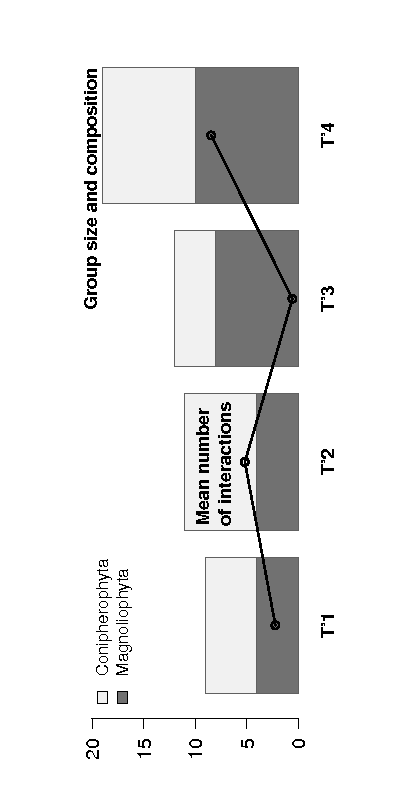
\includegraphics[height=.2\textwidth, width=.3\textwidth, trim=150 200 150 200, clip=]{\fignet/MRV10_AoAS_Q4_group} \\} 
      \onslide+<4->{\paragraph{Group interactions:} \\ 
        \includegraphics[height=.3\textwidth, width=.3\textwidth]{\fignet/Tree-adjMat-SBMtaxo}} 
    \end{tabular}    
  \end{tabular}
  
}

%====================================================================
\frame{\frametitle{Some differences} 

  \paragraph{Nature of the latent variables:}
  \begin{itemize}
    \setlength{\itemsep}{1.25\baselineskip}
    \item \emphase{Species abundance =} continuous, multivariate (Gaussian)
    \item \emphase{Network =} univariate, discrete (multinomial)
  \end{itemize}
  
  \bigskip \bigskip \pause
  \paragraph{Modeling function of the latent variables:}
  \begin{itemize}
    \setlength{\itemsep}{1.25\baselineskip}
    \item \emphase{Species abundance =} instrumental: comfortable multivariate Gaussian setting \\
    \ra no precise ecological interpretation of the $Z_i$ \\
    \ra focus on the inference of the parameter $\theta = (\beta, \Sigma)$
    \item \emphase{Network =} 'mechanistic': hopefully, species groups have an ecological meaning \\
    \ra easier interpretation of the $Z_i$ \\
    \ra focus on unsupervised classification
  \end{itemize}
  
  \bigskip \bigskip \pause
  \paragraph{Many other typical uses of latent variable:} modelling time, space or time-space dependencies

}

%====================================================================
\frame{\frametitle{Latent variable models in ecology \refer{PeG22b}} 

  $$
  \begin{tabular}{cc}
%     \includegraphics[height=.6\textheight]{\fig/PeG22-Fr-BookCover} & 
    \includegraphics[height=.6\textheight]{\fig/PeG22-En-BookCover}
  \end{tabular}
  $$
  (French version: \refer{PeG22a}).

}



%====================================================================
%====================================================================
\section{Statistical inference}
\frame{\frametitle{Outline} \tableofcontents[currentsection]}
%====================================================================
\frame{\frametitle{Incomplete data models} 

  \paragraph{Reminder.}
  \begin{description}
  \item[$Y =$] observed variables (responses)
  \item[$X =$] \textcolor{gray}{observed covariates (explanatory: dropped for the sake of clarity)}
  \item[$Z =$] latent (= unobserved, hidden) variables
  \item[$\theta =$] unknown parameters
  \end{description}
  
  \pause \bigskip \bigskip
  \paragraph{Two inference frameworks.}
  \begin{itemize}
  \item Frequentist:
  \begin{align*}
  \text{latent variables} = \text{random, \qquad parameters} = \text{fixed}
  \end{align*}
  \item \pause Bayesian: 
  \begin{align*}
  \text{both latent variables and parameters} = \text{random}
  \end{align*}
  (still: \# latent variables $\simeq$ { \# data,} 
  {\# parameters } $\ll$ { \# data})
  \end{itemize}

  \pause \bigskip \bigskip
  \paragraph{In both case:} Inference would be easy if $Z$ was observed.
  
}

%====================================================================
\frame{\frametitle{Frequentist setting} 

  Maximum-likelihood inference requires to deal with
  $$
  p_\theta(Y) = \int p_\theta(Y \mid Z) \d p_\theta(Z)
  $$

  \bigskip \bigskip \pause
  \paragraph{Most common approach.} Expectation-Maximization (EM) algorithm \refer{DLR77}:
  \medskip
  \begin{itemize}
    \setlength{\itemsep}{1.25\baselineskip}
    \item E step = determination of (some moments of)
    $$
    p_{\widehat{\theta}}(Z \mid Y)
    $$
    \item M step = update of $\widehat{\theta}$
  \end{itemize}
}

%====================================================================
\frame{\frametitle{Bayesian setting} 

  Aims at determining the {\sl posterior} distribution
  \begin{align*}
    p(\theta, Z \mid Y) 
    & = p(\theta \mid Y) p(Z \mid \theta, Y) \\ 
    & = p(Z \mid Y) p(\theta \mid Z, Y) 
  \end{align*}

  \bigskip \pause
  \paragraph{Similar issue.} Need to known something about
  \medskip
  \begin{itemize}
    \setlength{\itemsep}{1.25\baselineskip}
    \item either
    $$
    p(Z \mid Y)
    $$
    \item or
    $$
    p(Z \mid Y, \theta)
    $$
  \end{itemize}
}

%====================================================================
\frame{\frametitle{Conditional distributions} 

  \paragraph{Critical step:} evaluate \textcolor{gray}{(some moments of)} the conditional distribution $p_\theta(Z \mid Y)$ or $p(Z \mid Y, \theta)$

  \bigskip \bigskip 
  \paragraph{Three main cases.}
  \medskip
  \begin{itemize}
    \setlength{\itemsep}{1.25\baselineskip}
    \item \pause Easy cases: explicit \\
    \ra mixture models, simple mixed models, conjugacy, ...
    \item \pause Tricky cases: non-explicit
    , but still exact, ... \\ 
    \ra hidden Markov models, evolutionary models, belief propagation on trees... 
    \item \pause Bad cases: no exact evaluation \\
    \ra either sample from it (Monte-Carlo) \\
    \ra or approximate it (variational approximations)
  \end{itemize}

}

%====================================================================
\frame{\frametitle{Back to the two models} 

  \paragraph{Species abundance (PLN).} $Z_i =$ latent vector encoding species dependencies:
  \medskip
  \begin{itemize}
    \setlength{\itemsep}{1.25\baselineskip}
    \item $Z_i$ is marginally Gaussian, but not conditionally Gaussian
    \item No close form for $p_\theta(Z_i \mid Y_i)$ (even for $p = 1$ species)
  \end{itemize}

  \bigskip \bigskip \bigskip \pause
  \paragraph{Network (SBM).} $Z =$ latent group structure of the network:
  \medskip
  \begin{itemize}
    \setlength{\itemsep}{1.25\baselineskip}
    \item species memberships $Z_i$ are marginally independent, but not conditionally independent
    \item $p_\theta(Z \mid Y)$ defined over the $K^n$ possible configurations
  \end{itemize}

}

%====================================================================
\frame{\frametitle{Variational approximation} 

  \paragraph{Problem.} $p_\theta(Z \mid Y)$ being intractable, look for a 'good' approximation of it:
  $$
  q(Z) \approx p_\theta(Z \mid Y)
  $$

  \bigskip \bigskip \pause 
  More specifically, given
  \begin{itemize}
    \setlength{\itemsep}{1.25\baselineskip}
    \item \emphase{a set of approximating distributions $\Qcal$} and
    \item \emphase{a divergence measure $D[q \,\|\, p]$},
  \end{itemize}
  \pause \bigskip take
  $$
  q^* = \argmin_{q \in \emphase{\Qcal}} \; \emphase{D}\left[q(Z) \,\|\, p_\theta(Z \mid Y)\right]
  $$

  \bigskip \bigskip \pause 
  \paragraph{Most common choice for $D$ =} K\"ulback-Leibler divergence \refer{BKM17}
  $$
  D\left[q(Z) \,\|\, p_\theta(Z \mid Y)\right] = KL\left[q(Z) \,\|\, p_\theta(Z \mid Y)\right]
  $$
  but alternative choices exist \refer{Min05,WaJ08}
}

%====================================================================
\frame{\frametitle{Back to the two models} 

  \paragraph{Species abundance (PLN).} $Z_i =$ latent variable encoding species dependencies:
  \medskip
  \begin{itemize}
    \setlength{\itemsep}{1.25\baselineskip}
    \item $Z_i$ is marginally Gaussian, but not conditionally Gaussian, still, take \refer{CMR18a,CMR18b}:
    $$
    p(Z_i \mid Y_i) \approx q(Z_i) = \Ncal(Z_i; \widetilde{m}, \widetilde{S}_i)
    $$
  \end{itemize}

  \bigskip \bigskip \bigskip \pause
  \paragraph{Network (SBM).} $Z =$ latent group structure of the network:
  \medskip
  \begin{itemize}
    \setlength{\itemsep}{1.25\baselineskip}
    \item species memberships $Z_i$ are marginally independent, but not conditionally independent, still, take \refer{DPR08,MRV10}:
    $$
    p(Z \mid Y) \approx q(Z) = \prod_i q_i(Z_i)
    $$
    (mean-field approximation)
  \end{itemize}

}

%====================================================================
\frame{\frametitle{Variational Bayes} 

  \paragraph{Problem.} We look for the posterior
  $$
  p(\theta, Z \mid Y)
  $$
  where $\theta$ and $Z$ have no reason to be conditionally independent.
  
  \bigskip \bigskip \bigskip \pause
  \paragraph{Variational Bayes (VB).} Still, look for
  $$
  p(\theta, Z \mid Y) \approx q(\theta, Z) = q_1(\theta) q_2(Z).
  $$

}

%====================================================================
\frame{\frametitle{Variational approximation for latent variable models} 

  \paragraph{What do we gain?} 
  \medskip
  \begin{itemize}
    \setlength{\itemsep}{1.25\baselineskip}
    \item Something rather than nothing
    \item Good empirical results (in terms of bias, classification accuracy, ...)
    \item Computationally efficient algorithms (may deal with hundreds or thousands of species)
  \end{itemize}

  \bigskip \bigskip \pause
  \paragraph{What do we lose?} 
  \medskip
  \begin{itemize}
    \setlength{\itemsep}{1.25\baselineskip}
    \item Nothing as opposed to something
    \item Almost no statistical guaranty (consistency, asymptotic normality, ...) except for specific models (binary SBM without covariates)
    \item No or poor measure of uncertainty (VB tends to underestimate posterior variances, variational EM does not provide any)
  \end{itemize}
  
}


%====================================================================
%====================================================================
\section{Some attempts}
\frame{\frametitle{Outline} \tableofcontents[currentsection]}
%====================================================================

%====================================================================
\frame{\frametitle{Retrieving statistical guaranties} 

  \paragraph{Problem.}
  \begin{itemize}
    \setlength{\itemsep}{1.25\baselineskip}
    \item Variational approximations are nice and (reasonably) easy to implement
    \item But do not provide uncertainty measure (confidence/credibility interval, model uncertainty, ...)
  \end{itemize}
  
  \bigskip \bigskip \pause
  \paragraph{A possible approach:}
  Use variational approximations as a starting point for 
  \medskip
  \begin{itemize}
    \setlength{\itemsep}{1.25\baselineskip}
    \item statistically grounded but
    \item computationally demanding methods.
  \end{itemize}
  
}

%====================================================================
\frame{\frametitle{Model 2: Network model (with S. Donnet)} 

  \paragraph{Stochastic block model.} Models species interaction based on species similarity measures and assuming that species belongs to different groups ('blocks').
  
  \bigskip \bigskip \pause
  \paragraph{Variational EM} (VEM) algorithms are available for many block-models \refer{Leg16}.

  \bigskip \bigskip \pause
  \paragraph{Sequential Monte-Carlo} (SMC) is a well-established way to sample from the posterior, starting from a initial proposal distribution \\
  \ra The efficiency of SMC strongly relies on the choice of the initial proposal 
  
  \bigskip \bigskip \pause
  \paragraph{Combining both \refer{DoR21}.} 
  \begin{itemize}
    \setlength{\itemsep}{1.25\baselineskip}
    \item Derive a proposal $p_{start}(\theta, Z)$ from a frequentist VEM output
    \item Launch a classical SMC algorithm starting from $p_{start}(\theta, Z)$ to sample from $p(\theta, Z \mid Y)$.
  \end{itemize}

}

%====================================================================
\frame{\frametitle{Model 2: Sequential Monte-Carlo sampling} 

  \paragraph{Initial proposal} based on (approximate) frequentist inference: use (approximate) Louis formula \refer{Lou82} to get a starting value for $\Var(\theta \mid Y)$.
  
  \bigskip \pause
  \begin{tabular}{cc}
    \hspace{-.04\textwidth}
    \begin{tabular}{p{.5\textwidth}} 
      \paragraph{Principle.} \refer{DDJ06}
      \begin{itemize}
        \item \pause given $\textcolor{blue}{p_{{start}}(\theta, Z)}$
        \item \pause aiming at $\textcolor{red}{p_{{target}}(\theta, Z)} =  p(\theta, Z \mid Y)$ 
        \item \pause sample from a sequence of distributions
        $$
        \textcolor{blue}{p_{{start}} = p_0}, \; p_1, \; \dots, \; p_{H-1}, \; \textcolor{red}{p_H = p_{{target}}}
        $$
        with
        $$
        p_h(\theta, Z) \propto p_{{start}}(\theta, Z)^{{1 - \rho_h}} p_{{target}}(\theta, Z)^{{\rho_h}}
        $$
        and $0 = \rho_0 < \rho_1 \ < \dots < \rho_H = 1$
      \end{itemize}
    \end{tabular}
    &
    \begin{tabular}{p{.45\textwidth}}
      \includegraphics[width=.4\textwidth]{\figbayes/FigVBEM-IS-Tempering-4to2} \\
    \end{tabular}
  \end{tabular}
  
  \bigskip \pause
  \paragraph{Remark.} The step sizes $\rho_h$ can be chosen automatically at each step, to guaranty a sufficient effective sampling size (ESS).
  
} 


%====================================================================
\frame{\frametitle{Model 2: Tree interaction network} 

  \paragraph{Parameter posterior distribution} for $x = (\text{taxonomy, geography, phylogeny})$: 
  $$
  \begin{array}{ccc}
    \text{taxonomy} & \text{geography} & \text{phylogeny} \\
    \includegraphics[width=.25\textwidth]{\figbayes/DoR21-Fig7-beta1} & 
    \includegraphics[width=.25\textwidth]{\figbayes/DoR21-Fig7-beta2} & 
    \includegraphics[width=.25\textwidth]{\figbayes/DoR21-Fig7-beta3} \\
    \multicolumn{3}{l}{\text{Legend:} \qquad 
      \textcolor{red}{q_{VEM}(\beta_j)}, \qquad 
      \textcolor{darkgreen}{p(\beta_j \mid S, \widehat{K}(S), Y)}, \qquad 
      \textcolor{magenta}{p(\beta_j \mid S, Y)} }
  \end{array}
  $$
  
  \bigskip \pause
  \paragraph{Why so many steps} to go from \textcolor{red}{$q_{VEM}(\beta_j)$} to \textcolor{darkgreen}{$p(\beta_j \mid Y)$}?
  
  \bigskip 
  \hspace{-.025\textwidth}
  \begin{tabular}{rrrr}
    \paragraph{Correlation between estimates.} 
    & $(\beta_1, \beta_2)$ & $(\beta_1, \beta_3)$ & $(\beta_2, \beta_3)$ \\
    $p_{VEM}(\beta)$    & $-0.012$ & $ 0.021$ & $ 0.318$ \\
    $p(\beta \mid Y)$ & $-0.274$ & $-0.079$ & $-0.088$
  \end{tabular}
 
  \bigskip
  + $p(Z \mid Y)$ going away from $\prod_i q_i(Z_i)$.
}

%====================================================================
\frame{\frametitle{Model 1: Joint species distribution model (with J. Stoehr)} 

  \paragraph{Poisson log-normal model.} Joint species distribution model with gaussian latent layer to account for species dependencies.
  
  \bigskip \bigskip \pause
  \paragraph{Variational EM} (VEM) algorithm is available for PLN ({\tt PLNmodels} R package)

  \bigskip \bigskip \pause
  \paragraph{Monte-Carlo EM} (MCEM) is a stochastic alternative to EM, where the deterministic E step is replaced with a sampling step \\
  \ra The efficiency of MCEM strongly relies on the proposal used for the sampling step
  
  \bigskip \bigskip \pause
  \paragraph{Combining both.} 
  \begin{itemize}
    \setlength{\itemsep}{1.25\baselineskip}
    \item Use the VEM approximate conditional $q(Z)$ as a first Gaussian proposal
    \item Then update the parameters of the Gaussian proposal at each iteration of the EM algorithm.
  \end{itemize}

}

%====================================================================
\frame{\frametitle{Model 1: Importance sampling} 

  \paragraph{Monte-Carlo EM.} Require to sample from $p_{\widehat{\theta}}(Z \mid Y)$, which, we know, is not Gaussian.

  \bigskip \bigskip \pause
  \paragraph{Importance sampling.} Sample $Z^m$ iid from a proposal $q$, then weight each draw with weight
  $$
  w^m = p_{\widehat{\theta}}(Y, Z^m) / q(Z^m)
  $$
  which we know how to compute.

  \bigskip \bigskip \pause
  \paragraph{Results.} 
  \begin{itemize}
    \setlength{\itemsep}{1.25\baselineskip}
    \item Works well (unbiased estimates, asymtotically normal confidence intervals, ...: see next)
    \item as long as the number of species is small: $p \leq 6, 7$
  \end{itemize}
  \bigskip
  \ra Importance sampling yields a poor ESS when sampling in a large dimension $p$.
}

%====================================================================
\frame{\frametitle{Model 1: MCEM for $p=5$ species} 

  \begin{tabular}{cc}
    \hspace{-.05\textwidth}
    \begin{tabular}{p{.3\textwidth}}
      \paragraph{Simulated data.}
      \begin{itemize}
        \setlength{\itemsep}{1.25\baselineskip}
        \item $n = 100$ sites
        \item $p = 5$ species
        \item $d = 3$ covariates
        \item $B = 100$ replicates
      \end{itemize}
      
      \bigskip
      \paragraph{Empirical distribution.}
      $$
      (\widehat{\beta}_{hj}^m - \beta_{hj}^*) / \sqrt{\widehat{\Var}\widehat{\beta}_{hj}}
      $$
      
    \end{tabular}
    & 
    \hspace{-.05\textwidth}
    \begin{tabular}{p{.6\textwidth}}
      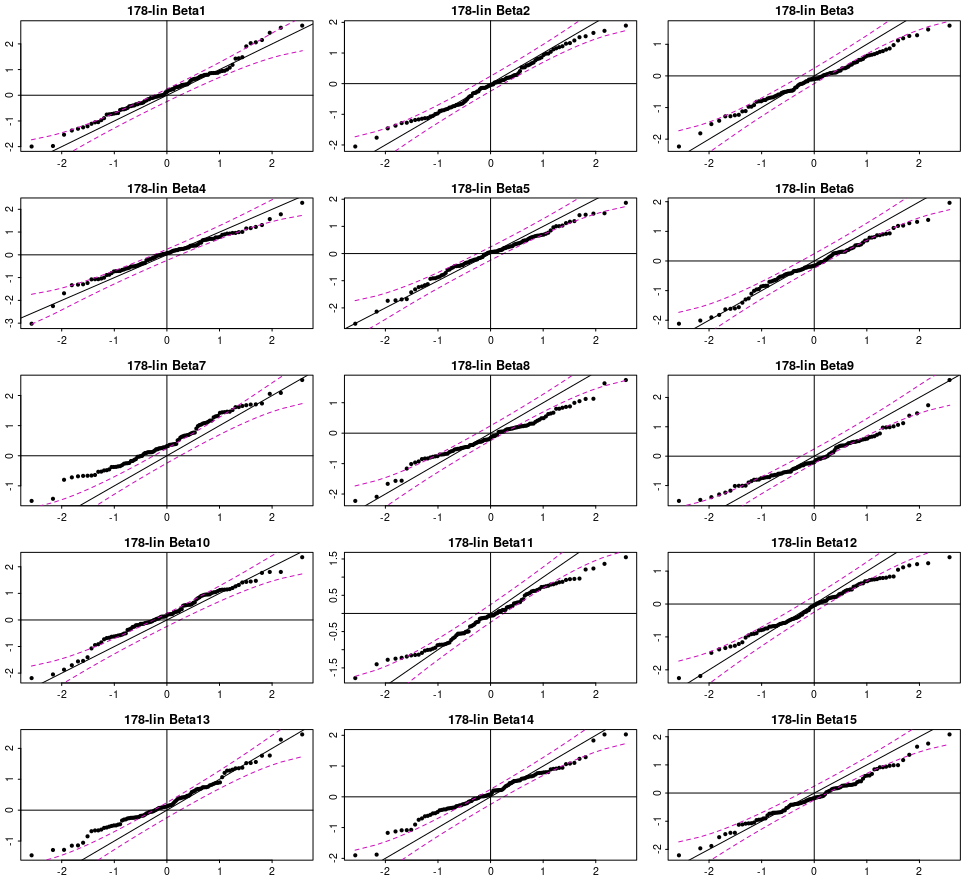
\includegraphics[width=.6\textwidth]{\fig/StR22-BetaHat-n100-d3-p5-parm1-nIS1000-lin-betaStat}
    \end{tabular}
  \end{tabular}

}


%====================================================================
\frame{\frametitle{Model 1: Composite likelihood} 

  \paragraph{The likelihood} is not the only admissible contrast for grounded statistical inference.

  \bigskip \bigskip \pause
  \paragraph{Composite likelihood} is one of the many others:
  \begin{itemize}
    \setlength{\itemsep}{1.25\baselineskip}
    \item build $B$ \emphase{overlapping} subsets of species, each with size $k$ (e.g. consider all pairs: $k=2$); 
    \item define the composite likelihood
    $$
    \cl_\theta(Y) = \sum_b \lambda_b \log p_\theta(Y^b); 
    $$
  \end{itemize}
  
  \bigskip \pause
  \paragraph{Guaranties}
  \begin{itemize}
    \setlength{\itemsep}{1.25\baselineskip}
    \item Under general conditions, $\widehat{\theta}_{CL} = \argmax_\theta \cl_\theta(Y)$ is consistent and asymptotically normal \refer{VRF11}.
    \item The (MC)EM algorithm can be adapted to the maximum composite likelihood estimation.
  \end{itemize}

}


%====================================================================
%====================================================================
\section*{Conclusion}
%====================================================================
\frame{\frametitle{Latent variable models in ecology} 

  \paragraph{Versatile modelling framework.} The latent layer can
  \medskip
  \begin{itemize}
    \setlength{\itemsep}{1.25\baselineskip}
    \item either encode some biologically meaningful structure
    \item or be mathematically convenient (e.g. to introduce dependence in the model)
  \end{itemize}

  \bigskip \bigskip \pause
  \paragraph{Statistical inference} not straightforward
  \medskip
  \begin{itemize}
    \setlength{\itemsep}{1.25\baselineskip}
    \item mostly because of unknown conditional distributions
    \item combinations of exact / sampling / approximate techniques seem promising
  \end{itemize}

  \bigskip \bigskip \pause
  \paragraph{Room for improvement} in many directions, especially in terms of
  \medskip
  \begin{itemize}
    \setlength{\itemsep}{1.25\baselineskip}
    \item computational burden
    \item efficiency in large dimension
  \end{itemize}

}



%====================================================================
\frame[allowframebreaks]{\frametitle{References} 

  {\tiny 
  \bibliography{/home/robin/Biblio/BibGene}
  \bibliographystyle{alpha}
  }

}

%====================================================================
\backupbegin
%====================================================================

%====================================================================
\backupend
%====================================================================

%====================================================================
%====================================================================
\end{document}
%====================================================================
%====================================================================
  
  \begin{tabular}{cc}
    \hspace{-.04\textwidth}
    \begin{tabular}{p{.5\textwidth}}
    \end{tabular}
    & 
    \hspace{-.02\textwidth}
    \begin{tabular}{p{.5\textwidth}}
    \end{tabular}
  \end{tabular}

